\documentclass[12pt]{article}
\usepackage[dvips]{epsfig}
\usepackage{color}
%e.g.  \textcolor{red,green,blue}{text}
\usepackage{url}
\usepackage[colorlinks=true]{hyperref}

\begin{document}

\section*{GENESIS: Documentation}

\section*{Project Browser Screenshots}

\begin{figure}[h]
  \centering
 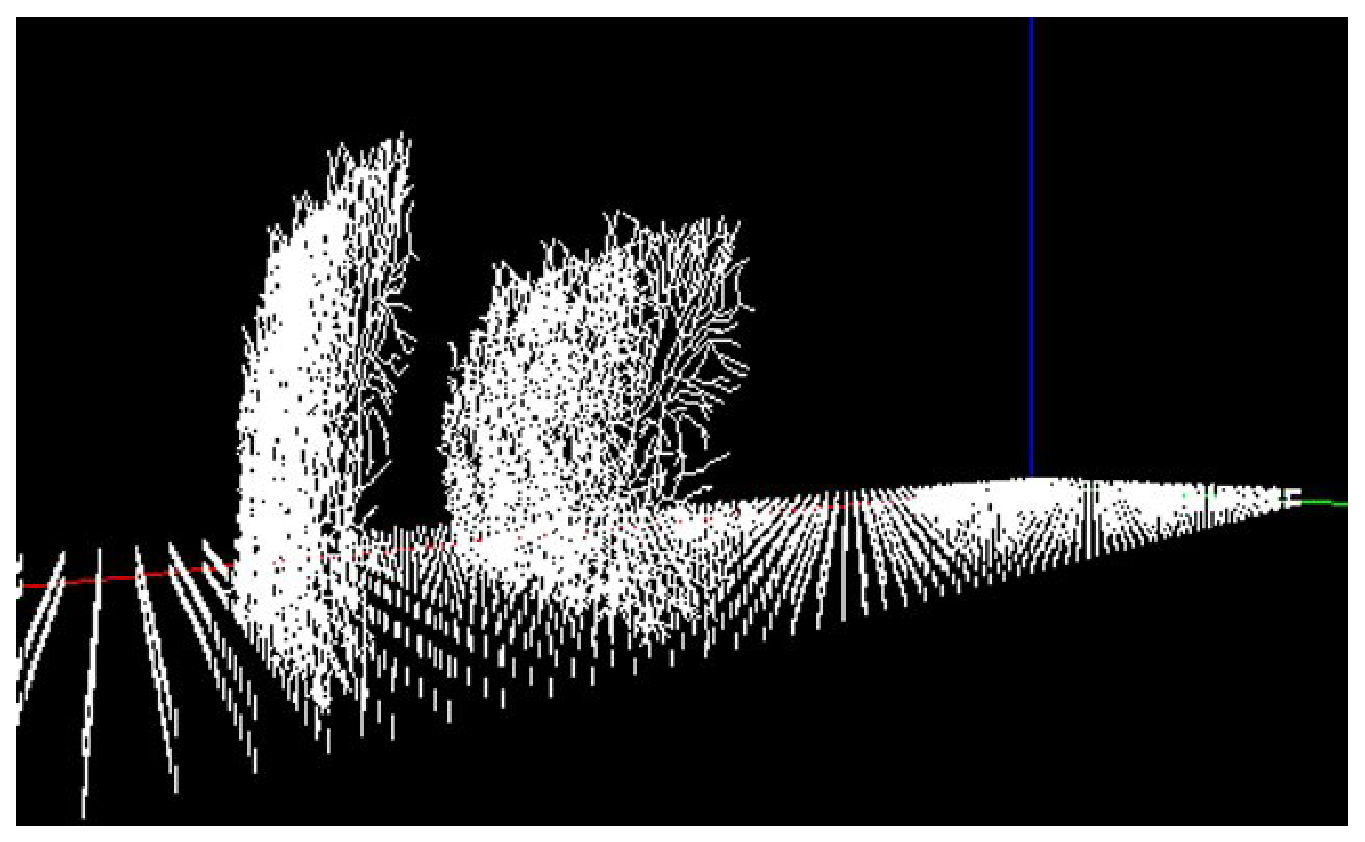
\includegraphics[scale=0.6]{figs/screenshot-1.eps}
%  \caption{{\bf Partial cerebellar cortex network :} 6 Purkinje and 6240 granule cells (330,000 equations)}
  \label{fig:pb-1}
\end{figure}

\begin{figure}[h]
  \centering
 
\includegraphics[scale=0.6]{figs/screenshot-2.eps}
%  \caption{{\bf Partial cerebellar cortex network :} 6 Purkinje and 6240 granule cells (330,000 equations)}
  \label{fig:pb-1}
\end{figure}

\begin{figure}[h]
  \centering
 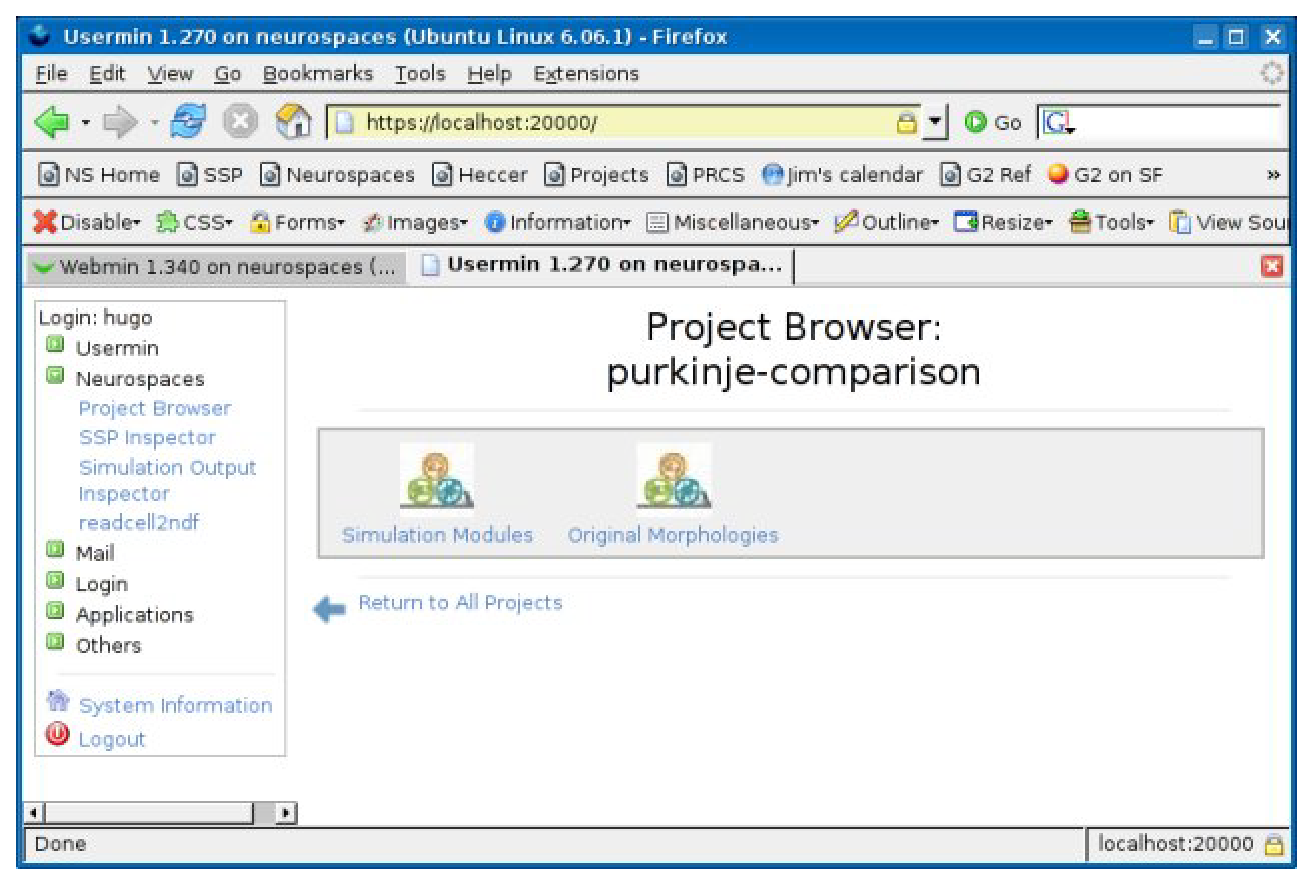
\includegraphics[scale=0.6]{figs/screenshot-3.eps}
%  \caption{{\bf Partial cerebellar cortex network :} 6 Purkinje and 6240 granule cells (330,000 equations)}
  \label{fig:pb-1}
\end{figure}

\begin{figure}[h]
  \centering
 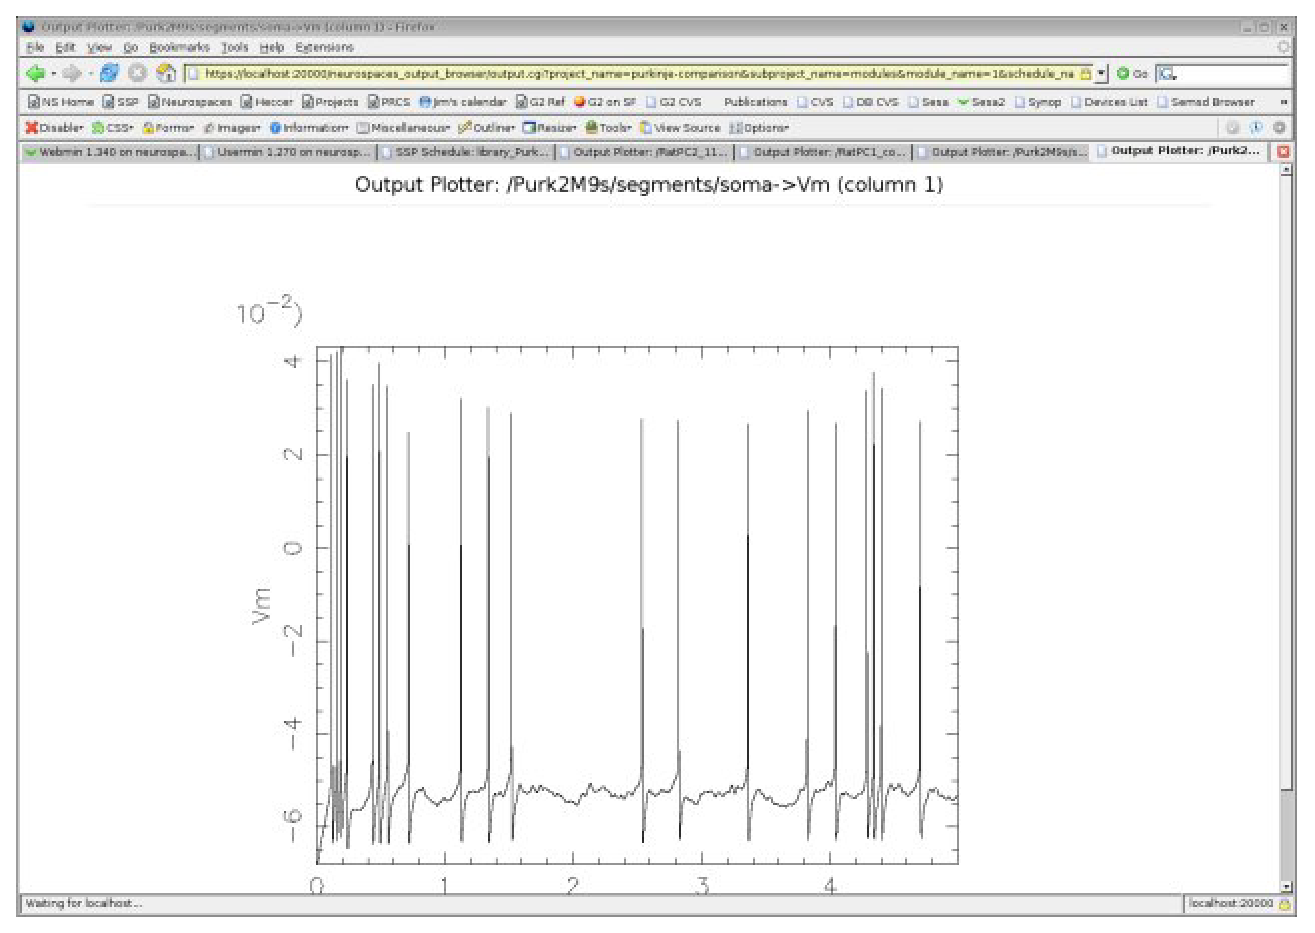
\includegraphics[scale=0.6]{figs/screenshot-4.eps}
%  \caption{{\bf Partial cerebellar cortex network :} 6 Purkinje and 6240 granule cells (330,000 equations)}
  \label{fig:pb-1}
\end{figure}

\begin{figure}[h]
  \centering
 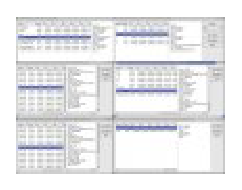
\includegraphics[scale=0.6]{figs/screenshot-5.eps}
%  \caption{{\bf Partial cerebellar cortex network :} 6 Purkinje and 6240 granule cells (330,000 equations)}
  \label{fig:pb-1}
\end{figure}

\begin{figure}[h]
  \centering
 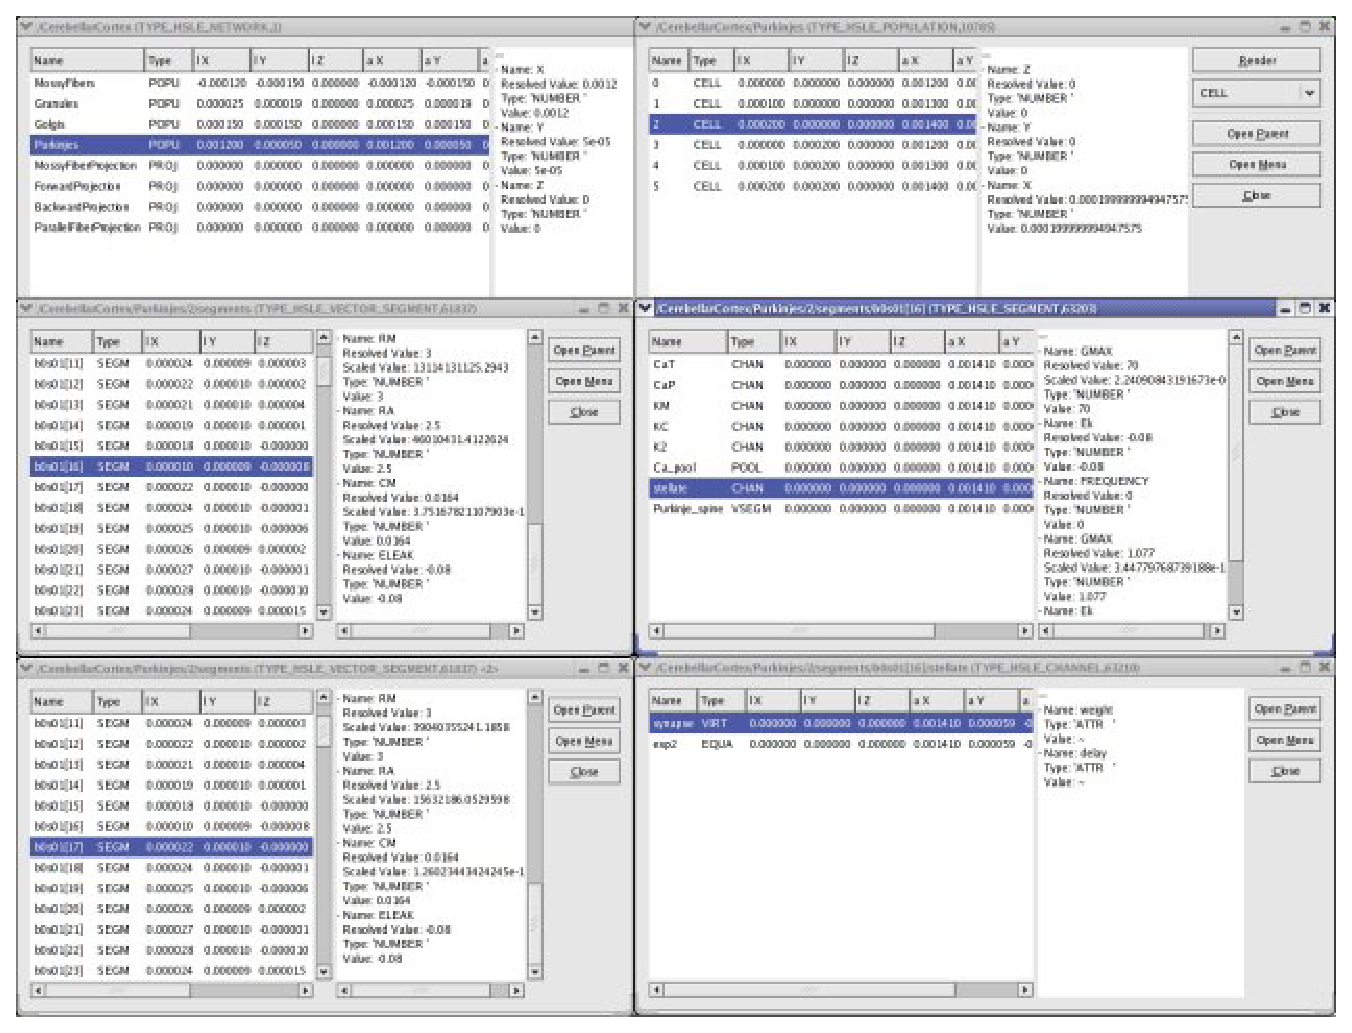
\includegraphics[scale=0.6]{figs/screenshot-6.eps}
%  \caption{{\bf Partial cerebellar cortex network :} 6 Purkinje and 6240 granule cells (330,000 equations)}
  \label{fig:pb-1}
\end{figure}

\end{document}
